\documentclass[review,preprint,12pt]{elsarticle}
%\biboptions{numbers,super,comma}
\biboptions{round,authoryear,semicolon}
\renewcommand{\cite}{\citep} % make default citations parenthetical

\usepackage{amsmath}
\usepackage{amssymb}
\usepackage{amsthm}

\usepackage{graphicx}
%\usepackage{natbib}
\usepackage{caption}
\usepackage{subcaption}

\usepackage{color}
\usepackage{soul}

\usepackage{diagbox}

%\biboptions{numbers,super,comma}

\newtheorem{theorem}{Theorem}[section]
\newtheorem{lemma}[theorem]{Lemma}

\theoremstyle{definition}
\newtheorem{definition}[theorem]{Definition}
\newtheorem{example}[theorem]{Example}
\newtheorem{xca}[theorem]{Exercise}

\theoremstyle{remark}
\newtheorem{remark}[theorem]{Remark}

\numberwithin{equation}{section}

%    Absolute value notation
%\newcommand{\abs}[1]{\lvert#1\rvert}

%    Blank box placeholder for figures (to avoid requiring any
%    particular graphics capabilities for printing this document).
\newcommand{\blankbox}[2]{%
  \parbox{\columnwidth}{\centering
%    Set fboxsep to 0 so that the actual size of the box will match the
%    given measurements more closely.
    \setlength{\fboxsep}{0pt}%
    \fbox{\raisebox{0pt}[#2]{\hspace{#1}}}%
  }%
}

\journal{Cell Systems}

\begin{document}

\begin{frontmatter}

\title{ %Exploiting redundancy in biological data to scale search tools with entropy \\
An entropy-scaling data structure for searching large-scale biological data}

%    Information for first author
\author[mitmath,mitcsail]{Y. William Yu\corref{co}}
\ead{ywy@mit.edu}
\author[mitmath,mitcsail]{Noah M. Daniels\corref{co}}
\ead{ndaniels@csail.mit.edu}
\author[mitcsail]{David C. Danko}
\ead{dcdanko@mit.edu}
\author[mitmath,mitcsail]{Bonnie Berger\corref{correspond}}
\ead{bab@mit.edu}
%    Address of record for the research reported here
\cortext[co]{These authors contributed equally to this work.}
\cortext[correspond]{Corresponding author}
\address[mitmath]{Department of Mathematics, Massachusetts Institute of Technology, Cambridge, Massachusetts 02139}
\address[mitcsail]{Computer Science and AI Lab, Massachusetts Institute of Technology, Cambridge, Massachusetts 02139}

%\email{bab@mit.edu}

%    General info
%\subjclass[2010]{Primary 68W99}

%\date{September 23, 2014}

%\dedicatory{This paper is dedicated to our advisors.}

%\begin{keyword}
%Similarity search, approximate matching, entropy scaling algorithms
%\end{keyword}

\begin{abstract}
    \begin{itemize}
        \item Low entropy data sets are common in Biological Big Data problems
        \item Under certain structural assumptions, it is possible to construct a data structure admitting similarity search in time- and space-complexity roughly linear to ``entropy''
        \item For problems drawn from genomics, small molecule search, and protein structure search, we demonstrate substantial acceleration of analyses using this data structure
    \end{itemize}
\noindent\unskip\textbf{eTOC Blurb}
\par\medskip\noindent\unskip\ignorespaces
Massive data sets in cell systems often exhibit high redundancy and thus low entropy.
We have developed a data structure for similarity search whose complexity scales with entropy.
This approach allows us to achieve massive acceleration of tools drawn from genomics, small molecule search, and protein structure search.
\end{abstract}

\end{frontmatter}

%\maketitle
\section{Summary}
{ \bfseries
    The continual onslaught of new data from cell systems has forced upon scientists the fortunate problem of having too much data to analyze.
    However, the standard toolkit of the modern practitioner, although sometimes sufficient, is ill-prepared to scale.
    Although computers are getting faster and cheaper, they are not doing so at a fast enough rate to keep pace with this exponential explosion of data.
    Luckily, it turns out that many of these huge data sets are highly 
redundant in nature, which researchers can exploit for the design of 
smarter tools for similarity search, the most fundamental task for analyzing 
biological data.
    In this paper, we introduce a novel entropy-scaling data structure---which scales in both time and space with the entropy of the underlying database---to perform similarity search.
    By applying this data structure---sometimes by itself and sometimes additionally exploiting additional domain-specific redundant structure in the database---we are able to achieve massive acceleration in several standard tools in the three domains of metagenomics, high-throughput drug screening, and protein structure search.
    In particular, we can achieve using our new entropy-scaling tools: CaBLASTX, 700x speedup of BLASTX with less than 5\% loss in sensitivity and no loss in specificity; Ammolite, \hl{??}x speedup of small molecule similarity search; and, Topaz, 2-30x speedup of FragBag with less than 0.2\% loss in sensitivity and no loss in specificity.
    Thus, we present not only a novel data structure for use in accelerating similarity search in low-entropy settings, but also practical tools ready for immediate use by the practitioner.

    All source code is publicly available for download at {http://gems.csail.mit.edu.}
}

\section{Introduction}
Throughout all areas of data science, scientists are being confronted by an 
explosion of data.
In many fields, and in particular molecular biology, this increase is exponential in nature, even outpacing Moore's and Kryder's laws on the respective doublings of transistors on a chip and long-term data storage density \hl{[cite]}.
As such, the challenges posed by the massive influx of data cannot be solved by waiting for faster and larger capacity computers, but require instead the development of data structures and representations that exploit and simplify complexity in the data set.

Here, we focus our attention on similarity search, where the task at hand is to find all entries in some database that are `similar', or approximate matches, to some query item.
Much like sorting is a primitive operation in computer science, similarity search is a fundamental operation in data science and lies at the heart of many other problems.
Traditionally, approximate matching has been studied primarily in the context of strings under edit distance metrics (e.g., for spell-checkers) \cite{ukkonen1985algorithms}.
However, similarity search has also demonstrated increasing importance in other biological system domains, including local alignment of sequences \cite{altschul1990basic, kent2002blat}, chemical graphs \cite{schaeffer2007graph}, and protein structures \cite{budowski2010fragbag}.
%In recent years, however, similarity search has become increasingly important for other objects and distance functions (e.g., biological genomes and alignment scores, networks and the Jaccard index) [Altschul et al, 1990; Kent, 2002; Schaeffer, 2007].

\begin{figure}[tbp]
    \centering
    \begin{subfigure}[b]{0.49\textwidth}
        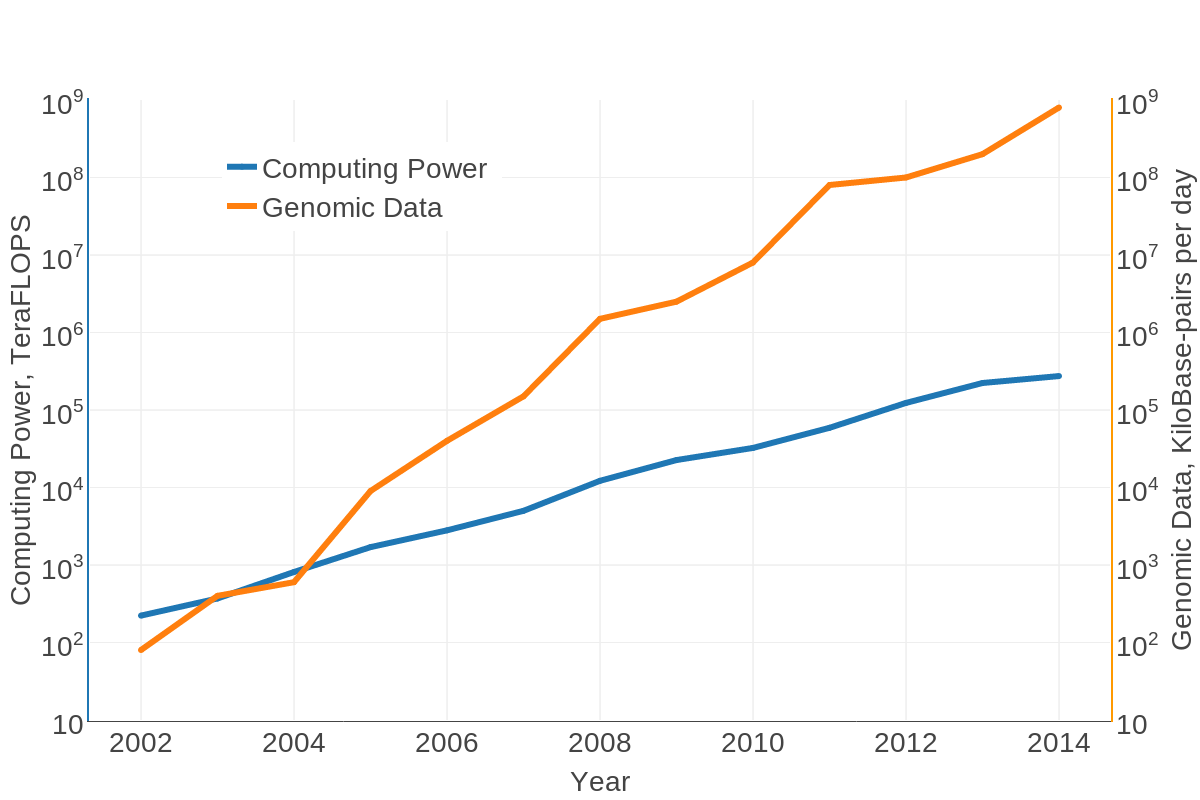
\includegraphics[width=1\textwidth]{assets/computeVsData.png}
        \caption{}
    \end{subfigure}%
    \begin{subfigure}[b]{0.49\textwidth}
        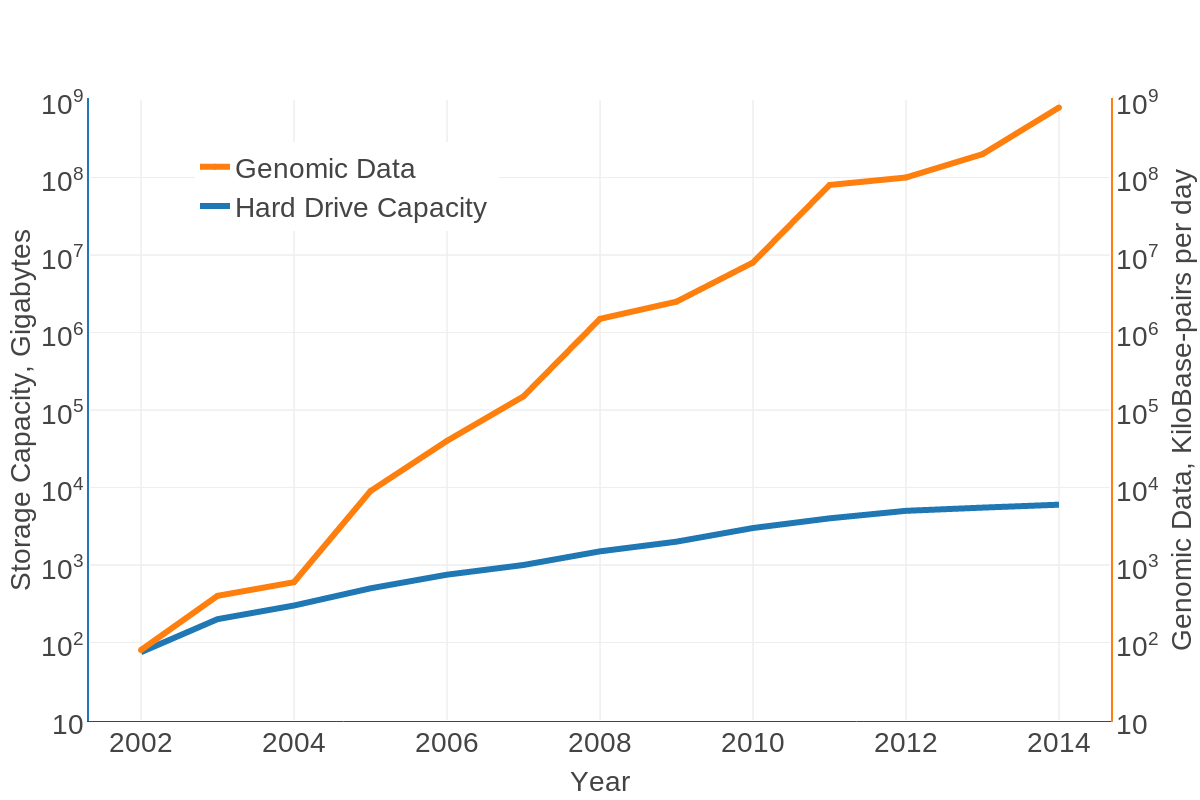
\includegraphics[width=1\textwidth]{assets/storageVsData.png}
        \caption{}
    \end{subfigure}
    \caption{Genomic data available has grown at a faster exponential rate than computer processing power and disk storage.}
    \label{fig:expdata}
\end{figure}

As available data grows exponentially \cite{berger2013computational,yu2015quality} (e.g., genomic data in Supplementary Figure S1), 
%move figure to supplement
algorithms that scale linearly with the amount of data no longer suffice.
The primary ways the literature addresses this problem (e.g.
locality sensitive hashing \cite{indyk1998approximate}, vector approximation \cite{ferhatosmanoglu2000vector}, space partitioning \cite{weber1998quantitative}) involve the construction of data structures that admit a more efficient search operation.
However, we note that as data increases, very often the redundancy present in the data also increases.
Existing general purpose methods do not explicitly exploit this particular feature of biological data.

In the specific context of local alignment in genomics, however, the emerging field of ``compressive genomics'' has shown that existing tools such as BLAST and BLAT can be ``compressively accelerated'' by taking advantage of high redundancy between related genomes using link pointers and edit scripts to a database of unique sequences \cite{loh2012compressive}.
Similar results have been demonstrated for local alignment in proteomics, using much the same strategies \cite{daniels2013compressive}.
Empirically, this compressive acceleration appears to scale almost linearly in the entropy of the database, often resulting in orders of magnitude better performance.

In this paper, we generalize this approach and introduce a practical opportunistic data structure for similarity search that provably scales almost linearly in both time and space with the entropy of the database.
Specifically, if similarity is defined by some metric-like distance function and the database exhibits both low `metric entropy' and low `fractal dimension', this data structure performs much better than na\"ive and even optimized methods.
This data structure allows for minimal (or even zero) loss in recall, coupled
with zero loss in specificity.
%We will define metric entropy and fractal dimension more precisely later, but intuitively, they are respectively measures of the total information content and scaling behavior of number of points contained in spheres of varying radii.
Although these `entropy-scaling data structures' can in principle be used to organize nearly any large data set for faster and more space-efficient analysis,
we demonstrate their utility on similarity search problems drawn from the three major biological `big challenges of big data': genomics, pharmaceuticals, and protein structure \cite{marx2013biology}.

\section{Results}
\subsection{Entropy-scaling data structure for similarity search}
\begin{figure}[btp]
    \centering
    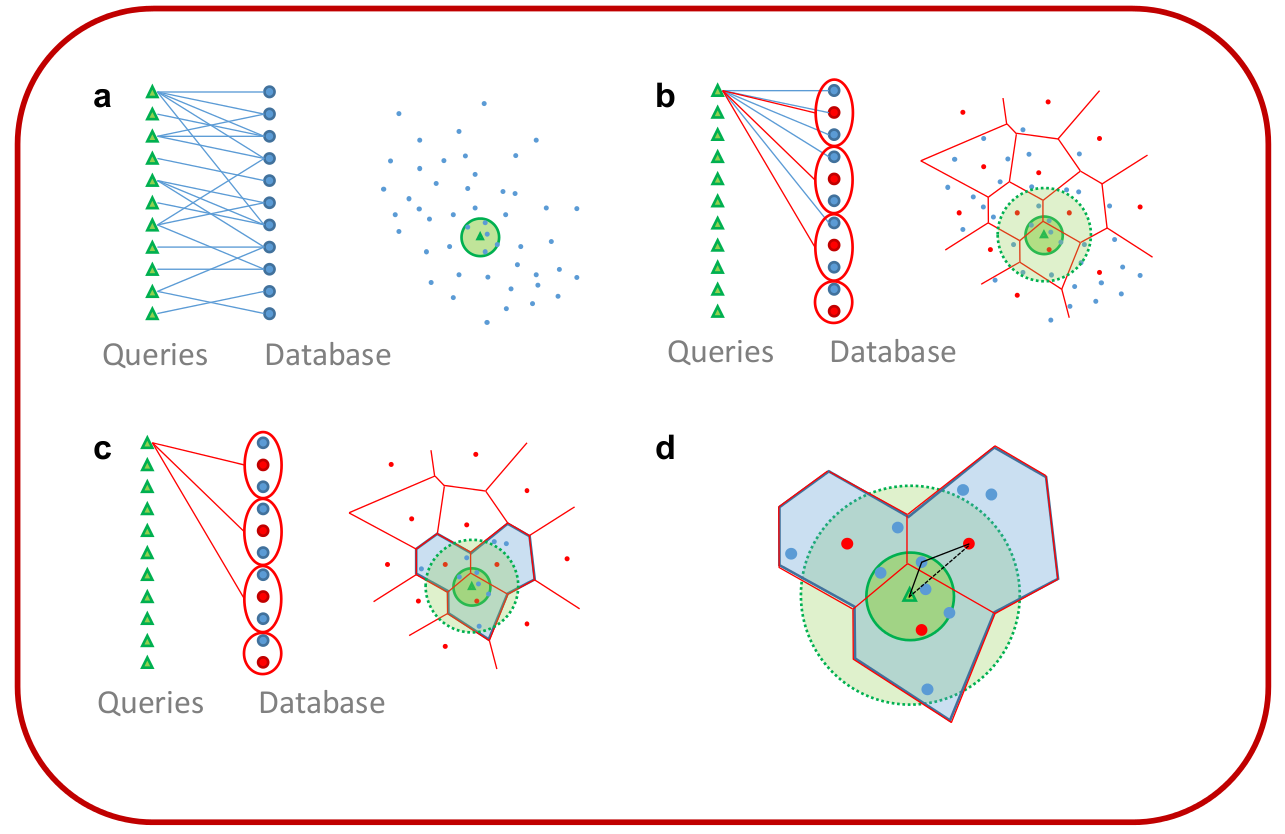
\includegraphics[width=1\textwidth]{assets/dataStructure.png}
    \caption{ Entropy-scaling data structure for similarity search. %
            (a) The na\"ive approach tests each query against each database entry to find entries within distance $X$  of the query. %
            (b) By selecting appropriate cluster centers with maximum radius $r_c$ to partition the database, we can (c) first do a coarse search to find all cluster centers within distance $r+r_c$ of a query, and then the (d) triangle inequality guarantees that a fine search over all corresponding cluster entries will suffice.}
    \label{fig:dataStructure}
\end{figure}

We present here an opportunistic data structure for similarity search that scales with the entropy of the underlying database.
In the following we consider entropy to be nearly synonymous with distance between points in a high-dimensional space.
For genomic sequences, this can be edit distance, for chemical graphs, maximum common subgraph size, and for general vectors, Euclidean or cosine distance.
The similarity search problem we are most interested in is finding all points in a set that are close to (i.e. similar to) the query point.
The basics of the data structure itself are presented in Figure \ref{fig:dataStructure}, but understanding why it works requires a bit more intuition.

Let's first consider what it means for a large biological data set, considered as points in a high-dimensional space, to be highly redundant.
Perhaps many of the points are exact duplicates; this easy scenario is trivially exploited by de-duplication and is already standard practice (e.g. the NR NCBI protein database \cite{pruitt2005ncbi}).
Or maybe the points mostly live on a low-dimensional subspace; statistical tools such as PCA (Principal Component Analysis) exploit this property in data analysis.
Furthermore, if the dimension of the subspace is sufficiently low and each dimension sufficiently ``long'',
the space can be divided into cells, allowing quick similarity searches by searching only nearby cells \cite{weber1998quantitative}.
However, when the dimensionality of that subspace increases, cell search time blows up exponentially, and in sparse data sets, most of the cells will be empty, which wastes search time.
Also, cell search performs poorly when each of the dimensions is small and discrete, as is the case with genomic sequences when we consider each position as a dimension and the four possible nucleotides as the possible locations along that axis.


\begin{figure}[btp]
    \centering
    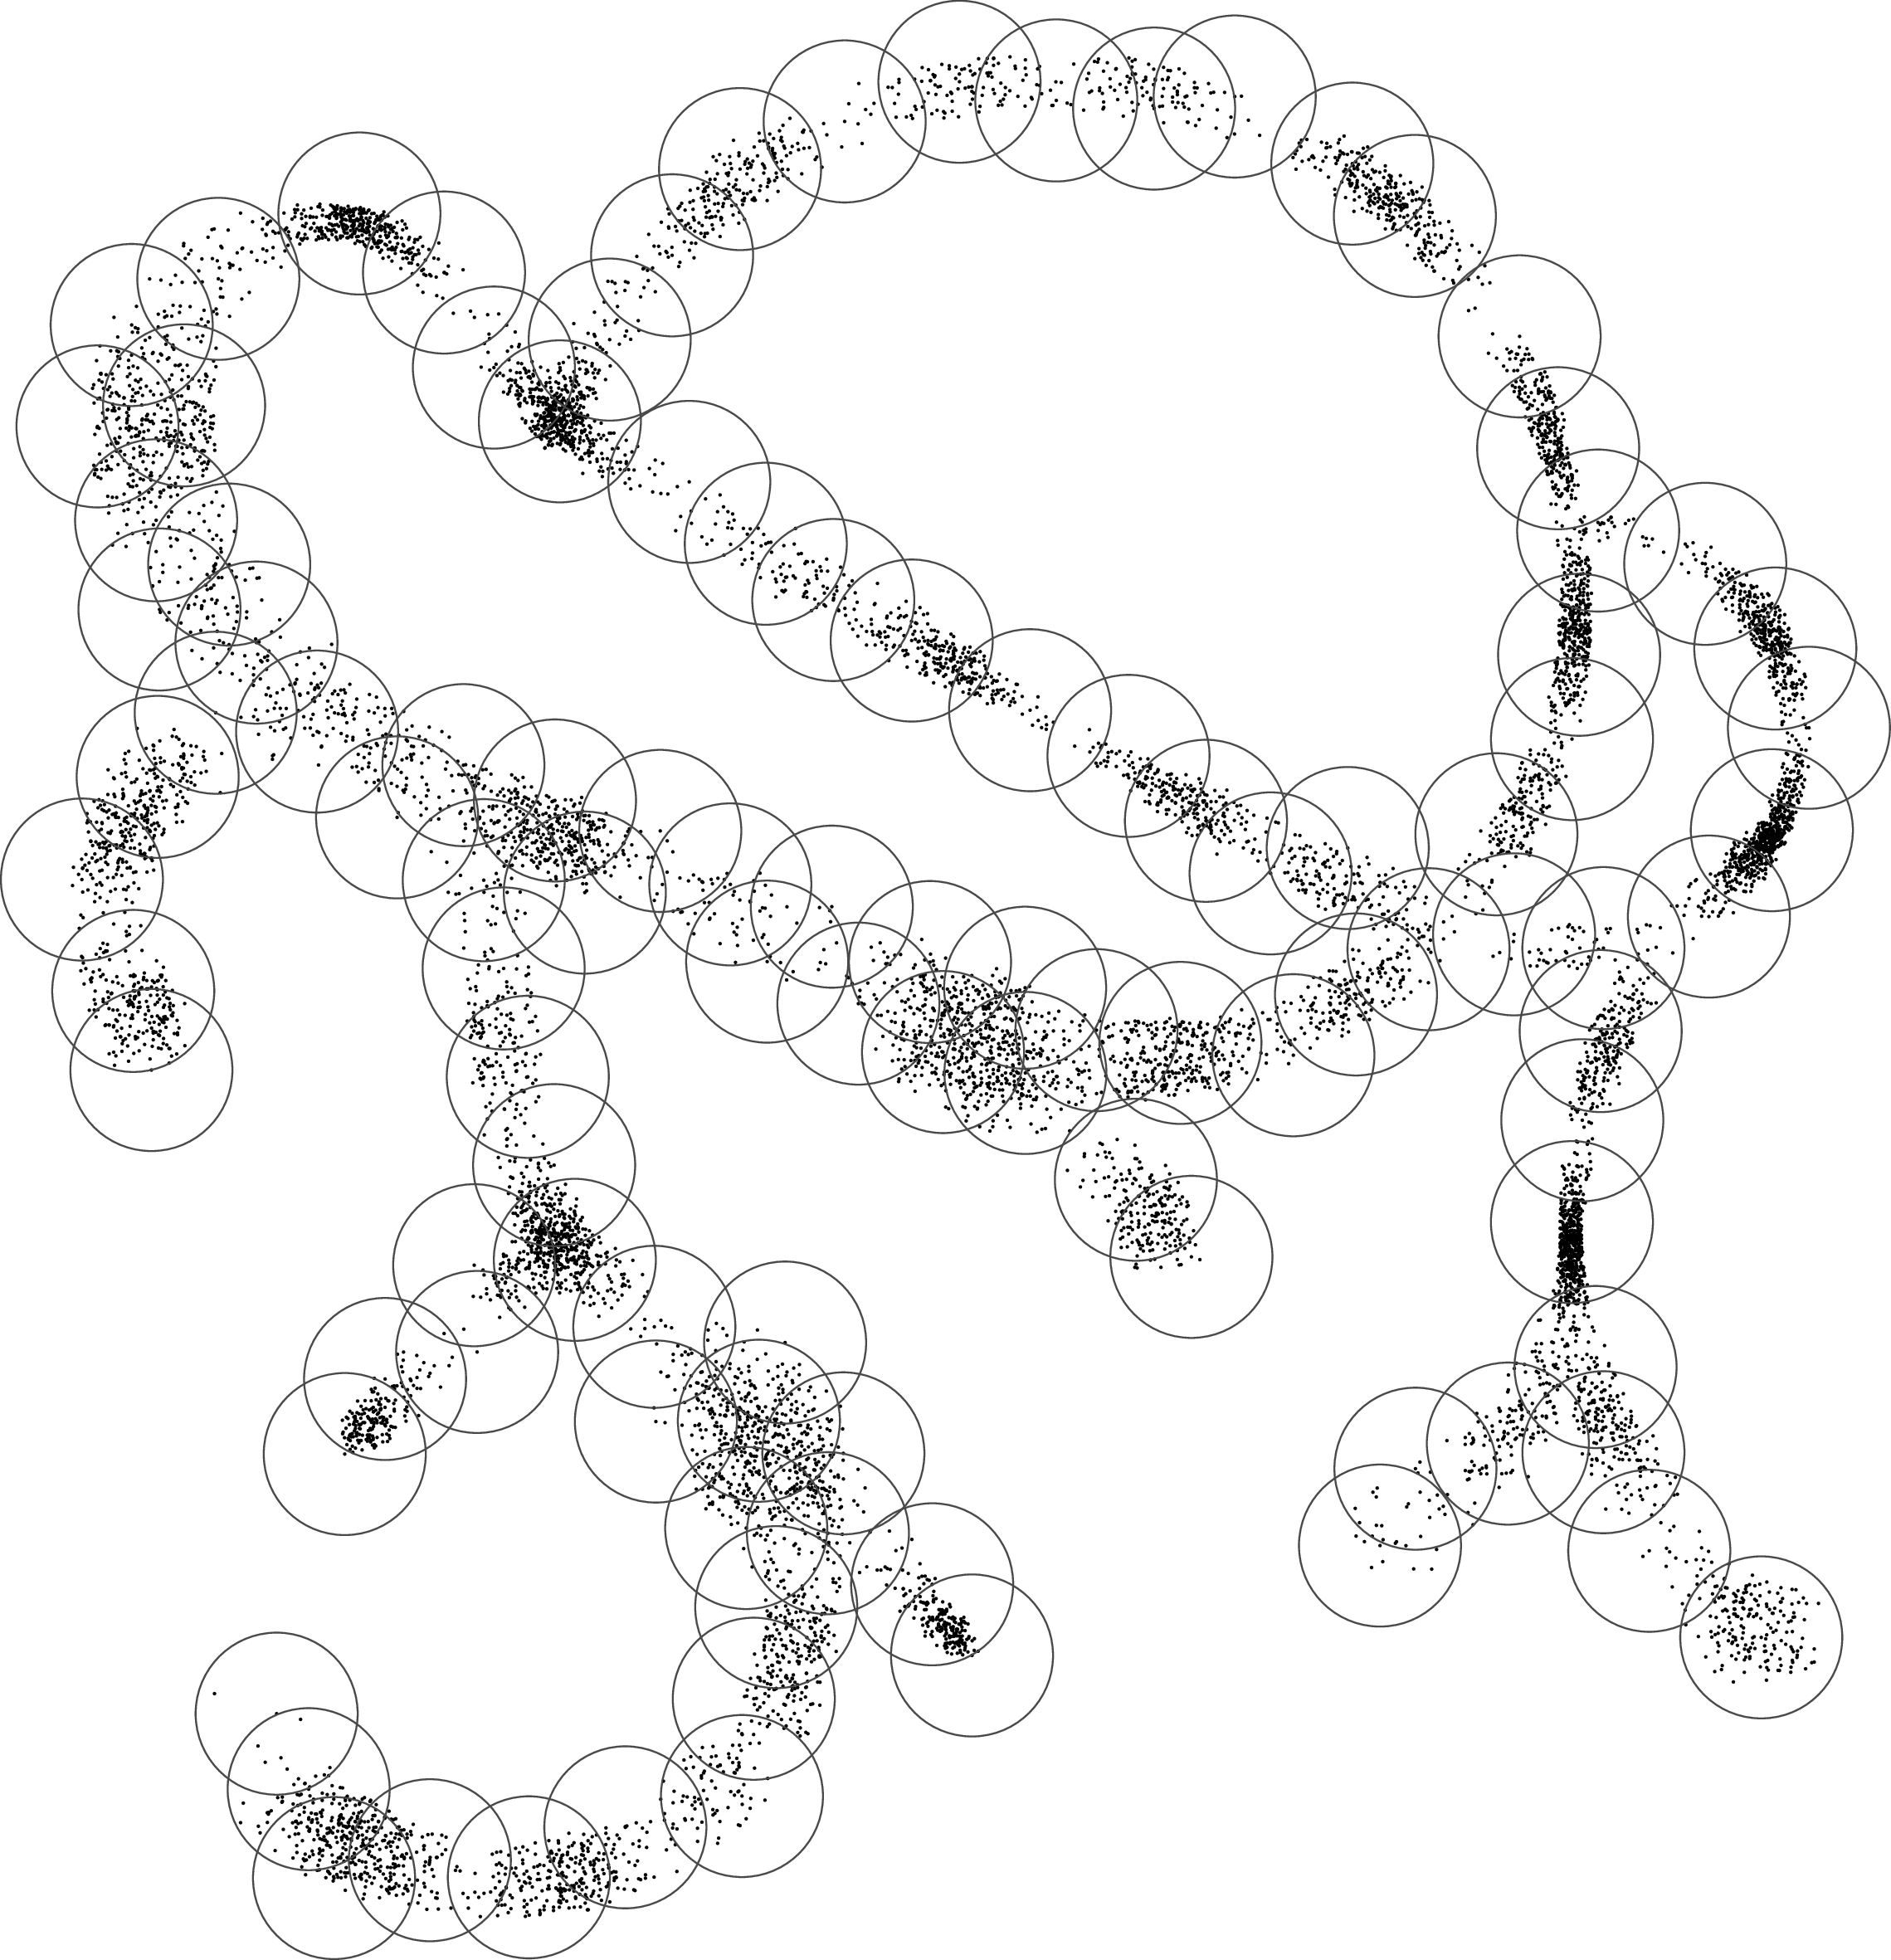
\includegraphics[width=0.8\textwidth]{assets/treepoints/treepoints2D_clusters.png}
    \caption{Cartoon depiction of points in a high-dimensional space that live close to a 1D tree-like structure. Although high-dimensional at a fine scale, at the coarser scale of covering spheres, the data cloud looks nearly 1-dimensional. Note that the cluster center generation was performed using the same algorithm used in Topaz, which is our accelerated version of FragBag.}
    \label{fig:tree}
\end{figure}
More importantly though, biological databases do not often actually live in low-dimensional subspaces.
Let's consider the instructive case of genomes along an evolutionary Tree of Life (Figure \ref{fig:tree}).
Such a tree has many branches (plus admixture merges branches back together), and might look nearly ``1-dimensional'' locally, but on a global scale is anything but---at least considering it as a subspace.
Additionally, because of diffusion due to mutation, each of the branches is also ``thick'' (high-dimensional) when looked at closely.
%Figure 1b for illustration.
%Please look up Jinbo Xu and my work on Tree Decomposition in JACM.
% NMD: I'm familiar with TreePack, but not seeing how it's relevant.
Thus, considering this example as a low-dimensional \textit{subspace} is the wrong thing to do.
However, the local low-dimensionality can be exploited by looking on the right scales.
In particular, we use two different scales: a coarse scale in which the tree looks 1-dimensional locally and a fine scale where the branch width matters.
We cover the tree with spheres of radius $r_c$, on the order of the width of the branches; these spheres determine our clusters, and the number of them is the ``metric entropy'' of the tree.
Because all the points within a sphere are close to each other, they can be encoded in terms of one another, and so are highly redundant; thus, the number of such spheres is a good approximation of the entropy of the entire database.

For any similarity search query looking for all points within distance $r$ of a query, by the triangle inequality, we need only look in nearby spheres with centers within a distance $r+r_c$ of the query.
%ref Figure 1?.
However, because the spheres have radius comparable to branch width, the tree is locally 1-dimensional on the coarse scale---we will call this the ``fractal dimension'' of the tree at the scale $r_c$.
Thus, doubling a search radius (or increasing from $r$ to $r+r_c$) only doubles (or increases by a factor of $\frac{r+r_c}{r}$) the number of points that need to be searched in a fine search after spheres have been identied.
Total similarity search time is then proportional to the number of spheres (the metric entropy) plus a constant multiple of the actual output size.

We have only considered here graph-like structures (i.e. an evolutionary tree), which are locally 1-dimensional.
However, the general scheme of covering the data set with spheres to then perform a coarse and fine search works even when the fractal dimension is higher (e.g. the local structure might be a 2D manifold).
All that will change is that the search time will have a component that blows up with increasing search radius by a function exponential in that fractal dimension.
However, assuming low fractal dimension, search time is still dominated by the metric entropy of the database.
Similarly, using these covering spheres, the database can be stored in a 
compressed manner (see Online Methods for further details).

Since real data is often messier than the rosy picture painted here, we
explore the application of this data structure to actual data in several different incarnations.
Additionally, sometimes the distance function we are given is not a metric (e.g. cosine distance), and thus we do not get a triangle inequality guarantee of 100\% sensitivity;
sometimes some of the clusters are much larger than others, and sometimes what 
counts as a point is not entirely clear without domain knowledge.
However, the diversity of the applications we explore in this paper demonstrate that the general scheme works for massively accelerating similarity search in a robust set of different contexts.
We expect that so long as the data set exhibits both low entropy (many items are similar to one another, which is nearly always the case when the query is a simlarity search) and low fractal dimension (the data set has some much simpler structure generating it, such as an evolutionary tree), our entropy-scaling data structure has the potential to achieve massive speedup over more naive methods and significant speedup over even other highly optimized methods.

\subsection{Metagenomics}

Metagenomics, the study of genomic data sequenced directly from environmental
samples, has recently grown in popularity.
From studies of the human gut microbiome to seawater and soil samples,
metagenomics has contributed to improved understanding of how ecosystems recover
from environmental damage~\cite{tyson2004community}, how the human gut responds 
to diet
and infection~\cite{david2014host}, and even some surprising clues as to disorders 
such as Autism Spectrum Disorder~\cite{macfabe2012short}.

Massive amounts of metagenomic reads are generated every day from 
next-generation sequencing (NGS) machines.
Overall, the rate of NGS sequencing is growing at a greater exponential rate
than computing power~\cite{loh2012compressive}.
These metagenomic reads must be stored and analyzed to do further downstream
analysis such as abundance determination (e.g. 
MetaPhlAn~\cite{segata2012metagenomic}) 
and functional characterization (e.g. PICRUSt~\cite{langille2013predictive}).
 Months of computing time are often required to process data for these novel, 
large-scale sequencing studies.
These computational challenges are at present a barrier to widespread use of 
metagenomic data throughout biotechnology, which impacts genomic medicine and 
environmental genomics~\cite{frank2008gastrointestinal}.

One approach to making metagenomic analysis tractable is to
sequence only the 16S ribosomal subunit of the microbiota, which is sufficient
to identify clades of microbes present in a sample. 
However, this approach cannot detect small functional differences between 
closely-related strains. 
In order to detect such minor functional differences, tools such as BLAST can 
be used to map metagenomic sequence data onto a database of known genome
sequences.
More recently, tools such as Kraken~\cite{wood2014kraken} have provided 
significantly faster methods for this genome mapping analysis.
This approach, however, requires a reference genome for each organism of
interest to first be identified.

Alternatively, BLASTX is widely used, both directly for analysis, as well as in 
pipelines such as MetaPhlAn~\cite{segata2012metagenomic}, to map reads to 
protein databases.
The advantage of the BLASTX approach is that complete reference genomes are not
required; BLASTX can identify homologs, particularly in the case where the
nucleotide sequence identity is low but translated protein sequence identity
is higher~\cite{turnbaugh2006obesity, kurokawa2007comparative}.
However, because BLASTX must search a protein database for possible hits for
each nucleotide read from a metagenomic sample, it is computationally intensive.
For example, \citet{mackelprang2011metagenomic} reported that using BLASTX to 
map 246
million reads against the KEGG~\cite{kanehisa2000kegg} database required 
800,000 CPU hours at a supercomputing center.
Moreover, BLASTX's run time requirements scale linearly with the size of the 
full read dataset, and each year require exponentially more runtime to process 
the exponentially growing read data. 


We present caBLASTX (compressively accelerated BLASTX), an algorithm and 
software implementation that relies on the techniques of compressive 
acceleration~\cite{loh2012compressive, daniels2013compressive} to map 
metagenomic reads onto a protein database orders of magnitude faster than 
BLASTX.

CaBLASTX is useful for two of the most common metagenomic analysis tasks. 
The first of these is mapping assembled or partially-assembled
nucleotide sequences onto a protein database. 
When these query sequences have
little in common with one another, caBLASTX maps each sequence separately. 
Each sequence is first searched against the compressed database with a 
relatively permissive E-value threshold, called coarse search. 
Any resulting hits may represent many original sequences, so these putative 
hits are expanded, and the search and alignment is refined with a less 
permissive E-value threshold, called fine search.

The second task caBLASTX can accelerate is that of mapping short nucleotide
reads (generated by next-generation sequencing technology) to a protein
database. In this instance, there is typically high coverage of the metagenomes
being sequenced, typically 30x-200x coverage. CaBLASTX takes advantage of this
redundancy
by compressing the read set as well, obtaining an additional speed gain that is
proportional to the amount of redundancy in the read data.


We tested caBLASTX on 200-400nt partially-assembled human gut microbiome
sequences, as well as on 151nt human gut microbiome reads at ~100x coverage.
For the partially-assembled sequences, we demonstrate run-time performance
approximately 10x faster than BLASTX, with negligible loss in sensitivity and
no loss in specificity. For the short reads, we demonstrate run-time
performance approximately 700x faster than BLASTX, with less than 5\% loss in
sensitivity and no loss in specificity.

CaBLASTX is a drop-in replacement for BLASTX in any pipeline.
As such, it can be used to accelerate other metagenomic analysis tools, such
as MetaPhlAn~\cite{segata2012metagenomic}.
Moreover, many of these analysis tools have, for performance reasons, required
users to construct a targeted protein database, which is a time-consuming and
possibly error-prone task.
However, caBLASTX makes it feasible to use the entire NCBI ``NR'' database for
analysis.

\subsubsection{Clustering}

CaBLASTX extends the approach of~\cite{daniels2013compressive} in order to 
cluster protein sequences.
Amino acid sequences are reduced from a 20-letter alphabet to a 4-letter
alphabet, which exposes more similarity among sequences at lower computational
cost.
This alphabet reduction can be thought of as a form of clustering; the offset 
within each of the 4 letters of the reduced alphabet is stored, so the original
sequence is recoverable (see Online Methods).
CaBLASTX employs a seed-and-extend approach in order to identify similar regions
of subsequence among entries in the database (see Online Methods).
This approach differs from the strict clustering described in the Data 
Structures section; in order to take advantage of the evolutionary nature of
protein sequence, \emph{subsequence} clustering is employed.
Specifically, CaBLASTX does not require that two entire protein sequences be 
similar in order to represent one in terms of the other; a similar region that 
is long enough (specifically, 40 residues at 70\% sequence identity in the 
reduced alphabet) will result in clustering of those subsequences. 
Thus, a sequence may have sub-sequences in a number of different clusters.

Given a clustering, each subsequence is represented in terms of a 
\emph{coarse sequence}, a pointer to the indices within the original sequence,
and the information required to recover the original sequence based on the
reduced alphabet.
Here, the distance function chosen, sequence identity based upon an alignment,
is decidedly not a metric.
In practice, however, as demonstrated in~\cite{daniels2013compressive} and 
here, this results in effective clustering performance with negligible loss of 
accuracy in search.

\subsubsection{Query Clustering}

Metagenomic reads are themselves nucleotide sequences, so no alphabet reduction
is performed on them directly.
Instead, metagenomic reads are compressed using the same approach as the
protein database, without the alphabet reduction step and with a number of
different parameters.
The difference scripts for metagenomic reads do not rely on the cluster offsets,
but simply store the substituted nucleotides.
Furthermore, unlike protein databases, where most typical sequences range in 
length from 100 to over 1000 amino acids, next-generation sequencing reads are 
typically short and usually of fixed length, which is known in advance.
Thus, the minimum alignment length required for a match, and the maximum
length unaligned fragment to append to a match, require different values based
on the read length.
An additional complication is that insertions and deletions from one read to
another will change the reading frame, potentially resulting in significantly
different amino acid sequences.
For this reason, query clustering requires long, \emph{ungapped} windows of high
sequence identity.
Specifically, for 202-nucleotide reads, for two sequences to cluster together,
we required a 150-nucleotide ungapped region of at least 80\% sequence identity.
Effectively, this means that the distance function for query clustering is
Hamming distance.
In the future, we may consider first translating the reads, and performing
clustering in the amino acid space (after alphabet reduction).
This would have the advantage of allowing reads with insertions or deletions
to cluster together, without causing reading-frame mismatches.
However, gapped alignment is significantly slower than ungapped alignment,
so the resulting cost of query clustering might negate speed gains.

We note that unlike the compression of the database, which can be amortized 
over future queries, the time spent clustering and compressing the queries 
cannot be amortized.
Thus, we would not refer to the query clustering as entropy-scaling, but it
still provides a practical benefit.


\subsubsection{Search}

Given a compressed protein database and a compressed query read set, search
comprises two phases.
The first, \emph{coarse search}, considers only the coarse sequences--the
representatives--resulting from compression of the protein database and the
query set.
Just as with standard BLASTX, each coarse nucleotide read is transformed into 
each of the six possible amino acid sequences that could result from it (three 
reading frames for both the sequence and its reverse complement).
Then, each of these amino acid sequences is then reduced back to a four-letter
alphabet using the same mapping as for protein database compression.
For convenience, the four-letter alphabet is represented using the standard
nucleotide bases, though this has no particular biological significance.
This is done so that the coarse search can rely on BLASTN (nucleotide BLAST) to
search these sequences against the compressed protein database.

This coarse search uses an E-value threshold that is relaxed from the one a user
specifies for the overall search, though the user can specify this coarse 
E-value threshold.
Coarse search identifies \emph{possible} hits for each query representative from
among the representative sequences in the database.
Of course, due to the reduced alphabet, some of these hits may turn out to be
poor quality when the original amino acid alphabet is considered.
Each of these coarse hits represents one or more original sequences from the
protein database; likewise, each coarse query represents one or more original
reads from the metagenomic data set.
For each coarse query representative, the set of coarse hits is used to
reconstruct all corresponding sequences from the original database by following
links to original sequence matches and applying their difference scripts.
The resulting \emph{candidates} are thus original sequences from the protein
database, in their original amino acid alphabet.
The query representative is also used to reconstruct all corresponding sequences
from the original read set.
Thus, for each coarse query representative, there is now a subset of the
metagenomic read set (the reads represented by that coarse query) and also a
subset of the protein database (the candidates).

The second phase, \emph{fine search}, uses standard BLASTX to translate each
of these reads associated with a coarse query representative and search for
hits only in the subset of the database comprising the candidates.
This fine search phase relies on a user-specified E-value threshold (defaulting
to BLASTX's default of 10) to filter hits.
To ensure that E-value calculation is correct, BLASTX uses a corrected database
size which is the size of the original, uncompressed protein database.

\subsubsection{Benchmarking}

To evaluate the run-time performance of caBLASTX, we tested it against
BLASTX as well as RapSearch2~\cite{zhao2012rapsearch2} and
Diamond~\cite{buchfink2014fast}.
BLASTX is often used to align assemblies thought to be exons to a protein
database, in which case metagenomic reads have already been assembled.
In this instance, the query-side compression of caBLASTX is not applicable, so
the performance gains are more modest.
We benchmarked caBLASTX vs. BLASTX on a dataset consisting of 22,778 assemblies
from human gut microbiota, 3.1 megabases in total, searching against the NCBI's
``NR'' non-redundant protein database from September, 2014.
The running time of BLASTX was 3235 minutes, compared to 123 minutes for caBLASTX, a speedup of 26.3.

When aligning unassembled next-generation sequencing reads to a protein 
database, the
query-side clustering aspect of caBLASTX becomes applicable.
We benchmarked caBLASTX against BLASTX on a set of 100,000
next-generation sequencing reads each of length 202 nucleotides from a human 
fecal dataset (SRR059854) from the
Human Microbiome Project~\cite{turnbaugh2007human}.
We filtered out reads starting or ending with 10 or more no-calls ('N').
The running time for BLASTX was 14,423 minutes, 
while caBLASTX took 21 minutes, a speedup of 673.
Results appear in Table~\ref{mgbench}.

\begin{table}
\caption{Comparison of caBLASTX and BLASTX running time and accuracy.\label{mgbench}}
\begin{tabular}{ccccc}
\hline
dataset & BLASTX (s) & caBLASTX  (s) & speedup & accuracy\\
\hline
assemblies & 3235 & 123 & 26.3x & 99.2\%\\
\hline
NGS reads & 14423 & 21 & 673x & 95.7\%\\
\hline
\end{tabular}
\end{table}



\subsubsection{Validation}

In order to validate caBLASTX's accuracy, we treated BLASTX as a gold standard. 
Since caBLASTX accelerates BLASTX
using entropy-scaling techniques, false positives with respect to BLASTX should 
not be possible, but false negatives certainly are.
We evaluated the hits from BLASTX and caBLASTX on the same human gut
assemblies and raw reads used for benchmarking, in order to evaluate the accuracy when
query-side compression is not used.
As false positive hits with respect to BLASTX are not possible, we report as 
accuracy the fraction of BLASTX hits that are also returned by caBLASTX.
We note that due to query-side compression, the output order from caBLASTX 
typically does not match that of BLASTX.
As show in Table~\ref{mgbench}, on the metagenomic assemblies, where query-side 
compression was not performed, caBLASTX achieves 99.2\% accuracy, while on the 
raw reads, caBLASTX achieves 95.7\% accuracy.


\subsection{High-throughput Drug Screening}

In the field of drug discovery and drug repurposing, prediction of biologically 
active compounds is a critical task. 
Computational high-throughput screening can eliminate many compounds from 
wet-lab consideration, but even this screening can be computationally 
intensive, and thus time-consuming.
PubChem~\cite{bolton2008pubchem} is a repository of molecular compound 
structures, 
which has grown exponentially since 2008 (Figure~\ref{pubchemdata}). 
In October, 2013, PubChem contained roughly 47 million molecular structures; 
in December, 2014 it contains 61.3 million structures.

We introduce a framework for clustering molecular databases that use the 
popular SDF molecular structure format, such as PubChem, and for searching for 
similar molecular structures in compressed space.
We designed this compression and search framework around one of the standard 
techniques for high-throughput screening of potential drug compounds, the use 
of maximum common subgraph (MCS) to identify similar motifs among molecules.
Many existing MCS-based tools, such as SMSD~\cite{rahman2009small} and 
fmcsR~\cite{cao2008maximum} compute the maximum common subgraph on fully 
labeled graphs; 
vertices are labeled with chemical elements, and edges are labeled with bond 
types (such as single or double bonds).
The `f' in fmcsR, which stands for ``flexible,'' indicates that some bounded 
number of vertex or edge label mismatches are permitted, at significant 
computational cost.

\subsubsection{Clustering}


Our clustering approach relies on structural similarity.
In order to more effectively group molecules based on structural motifs,
each molecule is \emph{simplified} by removing nodes and edges that do not
participate in simple cycles.
Clusters are formed of molecules that are isomorphic after this simplification
step.
Each cluster can then be represented by a single molecular structure, along 
with pointers to \emph{difference sets} between that structure and each of the 
full molecules it represents.
The difference set contains the nodes and edges that were removed in the 
simplification step.

\subsubsection{Search}

We implemented a variant of a maximum common subgraph (MCS) algorithm, known as 
\emph{flexible} maximum
common subgraph (fMCS), as detailed by Cao, et al.~\cite{cao2008maximum}.
Our implementation allows a user to specify whether any atom mismatches or 
bond-type mismatches should be 
allowed in the maximum common subgraph of two molecules.
If zero mismatches are allowed, fMCS is just MCS.
The distance function used is the graph distance metric 
of~\cite{bunke1998graph},
specifically $d(G_1,G_2) = 1 - \frac{|mcs(G_1,G_2)}{max(|G_1|,|G_2|)}$.

As in~\cite{loh2012compressive}, our compression-accelerated search approach 
relies on a two-stage process.
First, a \emph{coarse} search is performed in compressed space, by searching 
the coarse database.
The query molecule is simplified in exactly the same manner as 
the molecular database during clustering, and this transformed query graph is 
matched against the coarse database.
To preserve sensitivity, this coarse search is performed with a permissive 
similarity score.
The idea behind coarse search is to identify \emph{possible} hits.


Any possible hits--molecular graphs from the coarse database whose MCS to 
the transformed query molecule was within the similarity score threshold--are 
then reconstructed, by following
pointers to the removed atom and bond information, and recreating the 
original molecules.

Next, the \emph{fine search} is performed against these decompressed possible 
hits.
Fine search is performed using MCS or fMCS, with user-defined parameters for 
bond and atom mismatches and similarity-score threshold.

\subsubsection{Benchmarking}



\subsubsection{Validation}

\subsection{Protein Structure Search}

The relationship between protein structure and function has been a subject of intense study for decades,
and this strong link has been used for the fruitful prediction of function from structure \cite{hegyi1999relationship}.
To wit, given a protein of solved (or predicted) structure but unknown function, the efficient identification
of structurally similar proteins in the Protein Data Bank is critical to function prediction.
Relatedly, finding structural neighbors can also give insight into the evolutionary origins of proteins of interest.

One approach to finding structural neighbors is to attempt to align the query protein to all the entries in the Protein Data Bank (PDB) using a structural aligner (e.g. STRUCTAL \cite{subbiah1993structural} or ICE \cite{shindyalov1998protein}).
However, performing a full alignment against every entry in the PDB is prohibitively expensive, especially as the database grows.
Alternately, the approach we use here is the one introduced by FragBag~\cite{budowski2010fragbag}, which describes each protein as a
``bag of fragments,'' where each fragment is a small structural motif.

The bag of fragments is essentially
a term frequency vector representing the number of occurrences of each structural motif within the protein.
While FragBag does not generate structural alignments the way standard aligners do, it provides an excellent
filter for computing proteins that are likely to have close alignments; those alignments could then be computed
with a standard aligner.
FragBag's accuracy has been reported as comparable to structural aligners such as STRUCTAL and
ICE.
FragBag is already quite fast, much faster than these standard aligners, but also importantly for us
FragBag turns out to be very amenable to acceleration using an entropy-scaling data structure because much of the computation is spent in doing a similarity search on a frequency vector.

For this last example, we intentionally approached the application of entropy-scaling data structures to FragBag in a blind manner,
without using substantial domain-specific knowledge.
Instead, we used the very same representation (bag of fragments) and distance functions (Euclidean and cosine distances)
as FragBag, a greedy k-centers algorithm, and vector difference to generate the clustered representation.
Note that this is in stark contrast to caBlastX and Ammolite, which both exploited domain knowledge to further improve performance.
Thus, Topaz, our entropy-scaling version of FragBag, is exactly an existing FragBag codebase augmented with new database generation and similarity search functions.
Although it's conceivable that using similar techniques to exploit domain specific knowledge as in caBlastX and Ammolite will result in greater speedup, Topaz here is primarily a proof-of-concept to analyze the performance of a the entropy-scaling data structure alone.

\subsubsection{Clustering}
For the cluster generation, we used a randomized greedy 2-pass approach.
First, all proteins in the Protein Data Bank were randomly ordered.
Then in the first pass, proteins were selected as cluster centers if and only if they were not within a user-specified Euclidean distance $r_c$ from an existing center (i.e. the first protein is always selected, and the second if further away than $r_c$ from the first, etc.).
Recall that this generation of cluster centers is the same as the one used to generate covering spheres in Figure \ref{fig:tree};
the covering spheres were overlapping, but we trivially assign every protein uniquely to a single cluster by assigning to the nearest cluster center in the second pass.

\subsubsection{Search}
Similarity search here is performed exactly as described in the data structure section, with no modifications.
For a given search query $q$ and search radius $r$,
\begin{itemize}
    \item A coarse search is used to find all cluster centers within distance $r+r_c$ of $q$.
    \item All corresponding clusters were unioned into a set $F$.
    \item A fine search was performed over the set $F$ to find all proteins within distance $r$ of $q$.
\end{itemize}

\subsubsection{Benchmarking}
We explored the increases in speed resulting from applying the entropy-scaling data structure, for both Euclidean and cosine distances (Figure \ref{fig:fragbag}).
Naturally, as search radii increases, the coarse search expands to encompass the entire database; to fully explore parameters, we made certain to increase search radii until the acceleration effect entirely disappeared.
Additionally, we explored the effect of using different maximum cluster radii and several different query proteins.

For cosine distance, we generated databases with maximum cluster radii of 0.05, 0.1, 0.2, 0.3, 0.4, and 0.5.
Then, for each query protein from the set \{\texttt{4rhv}, \texttt{1ake}, \texttt{1bmf}, \texttt{1rbp}, \texttt{1b7t}\}, we ran both naive and accelerated similarity searches with radii of $0.02i \forall i \in \{0,\ldots,49\}$.
This was repeated 5 times for each measurement, and the ratio of average accelerated vs naive times is shown in Figure \ref{fig:fragbag_cosine}.

For euclidean distance, we generated databases with maximum cluster radii of 10, 20, 25, 50, and 100.
Again, for each query protein drawn from the same set, we compared the average over 5 runs of the ratio of average accelerated vs naive times (Figure \ref{fig:fragbag_euclid}.

As expected, the acceleration is highly dependent on both the search radius $r$ and the maximum cluster radius $r_c$.
Additionally, the query protein also makes a major difference in the results.
We suspect that this is due to the geometry of protein fragment frequency space being very ``spiky'' and ``star-like''.
Proteins that are near the core (and thus similar to many other proteins) show very little acceleration when our data structure is used because the majority of the database is nearby, whereas proteins in the periphery have fewer neighbors and are thus found much more quickly.
Changing the maximum cluster radius effectively makes more proteins peripheral proteins, but at the cost of overall acceleration.

Naturally, as the search radius expands, it quickly becomes necessary to compare against nearly the entire database, destroying any acceleration.
For the cosine space in particular, note that the maximum distance between any two points is $1$, so once the coarse search radius of $r+r_c >= 1.0$, there cannot ever be any acceleration as the fine search encompasses the entire database.
Similarly, once the coarse search encompasses all (or nearly all) the clusters in Euclidean space, the acceleration diminishes to 1x, and the overhead costs make the entropy scaling data structure perform worse than a naive search.
However, as we are most interested in proteins that are very similar to the query, the low-radius behavior is of primary interest.
In the low-radius regime, Topaz demonstrates varying though substantial acceleration (2x-30x) over FragBag.

Additionally, it is instructive to note that because of the very different geometries of euclidean vs cosine space, acceleration varies tremendously for some proteins, such as \texttt{4rhv} and \texttt{1bmf}, which display nearly opposite behaviors.
Whereas there is nearly 30x acceleration for \texttt{4rhv} in cosine space for low radius, and the same for \texttt{1bmf} in euclidean space, neither achieves better than $\sim$ 2.5x acceleration in the other space.

\begin{figure}[tbp]
    \centering
    \begin{subfigure}[b]{0.40\textwidth}
        \caption{Cosine distance}
        \label{fig:fragbag_cosine}
        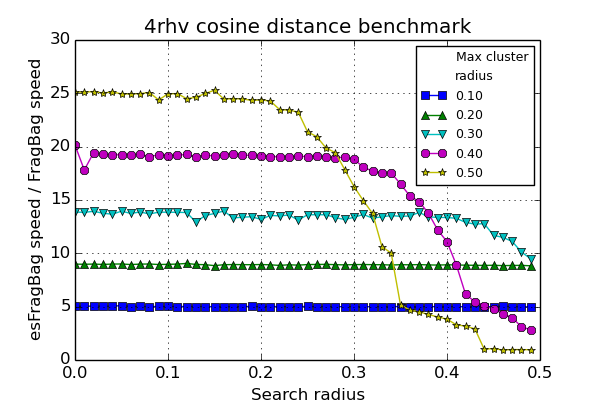
\includegraphics[width=1\textwidth]{assets/4rhv_cosine.png}
    \end{subfigure}%
    \begin{subfigure}[b]{0.40\textwidth}
        \caption{Euclidean distance}
        \label{fig:fragbag_euclid}
        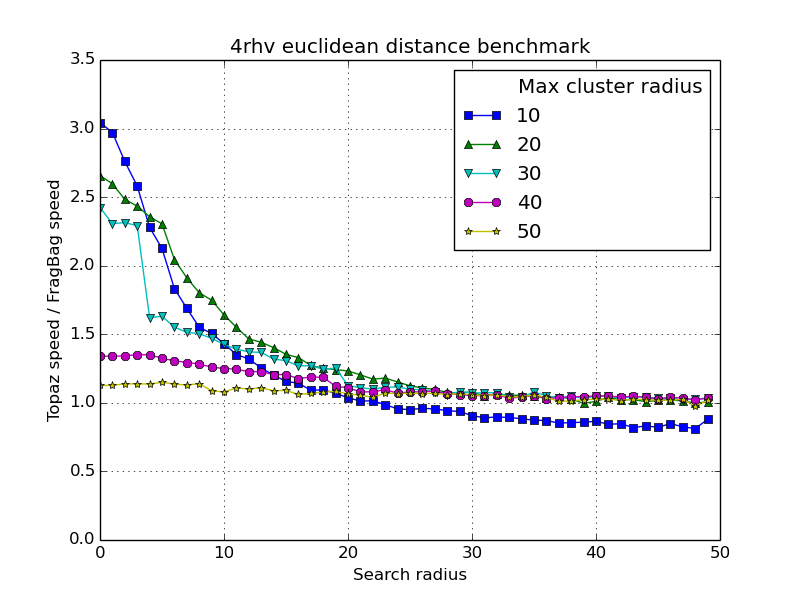
\includegraphics[width=1\textwidth]{assets/4rhv_euclid.png}
    \end{subfigure}
    \begin{subfigure}[b]{0.40\textwidth}
        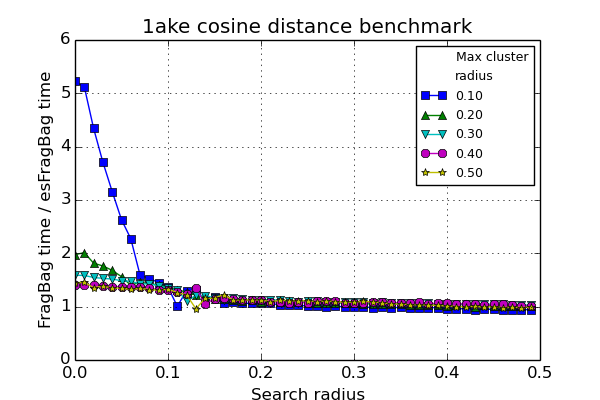
\includegraphics[width=1\textwidth]{assets/1ake_cosine.png}
        %\caption{}
    \end{subfigure}%
    \begin{subfigure}[b]{0.40\textwidth}
        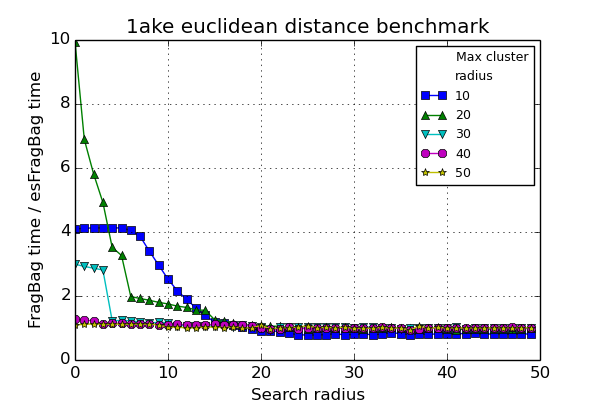
\includegraphics[width=1\textwidth]{assets/1ake_euclid.png}
        %\caption{}
    \end{subfigure}
    \begin{subfigure}[b]{0.40\textwidth}
        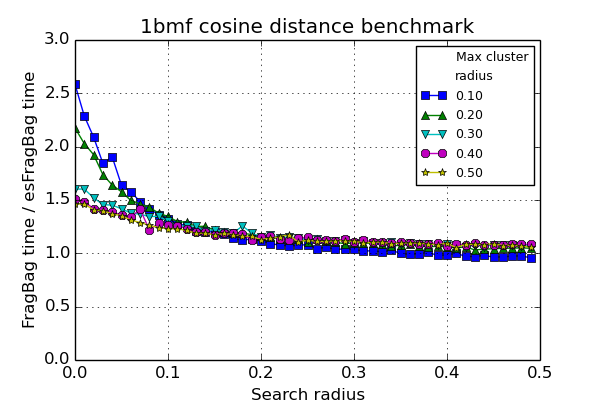
\includegraphics[width=1\textwidth]{assets/1bmf_cosine.png}
        %\caption{}
    \end{subfigure}%
    \begin{subfigure}[b]{0.40\textwidth}
        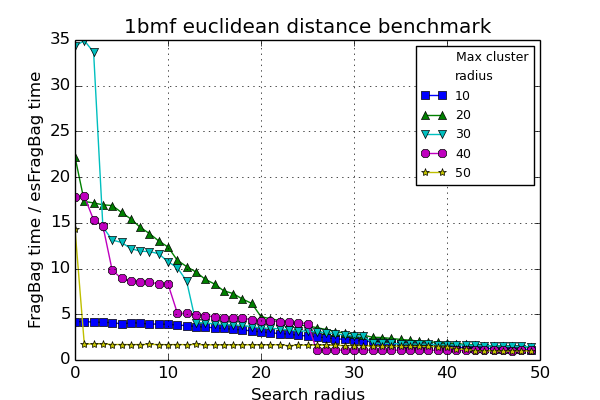
\includegraphics[width=1\textwidth]{assets/1bmf_euclid.png}
        %\caption{}
    \end{subfigure}
    \begin{subfigure}[b]{0.40\textwidth}
        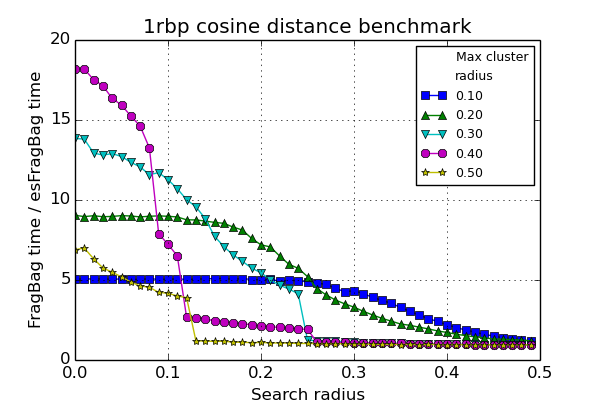
\includegraphics[width=1\textwidth]{assets/1rbp_cosine.png}
        %\caption{}
    \end{subfigure}%
    \begin{subfigure}[b]{0.40\textwidth}
        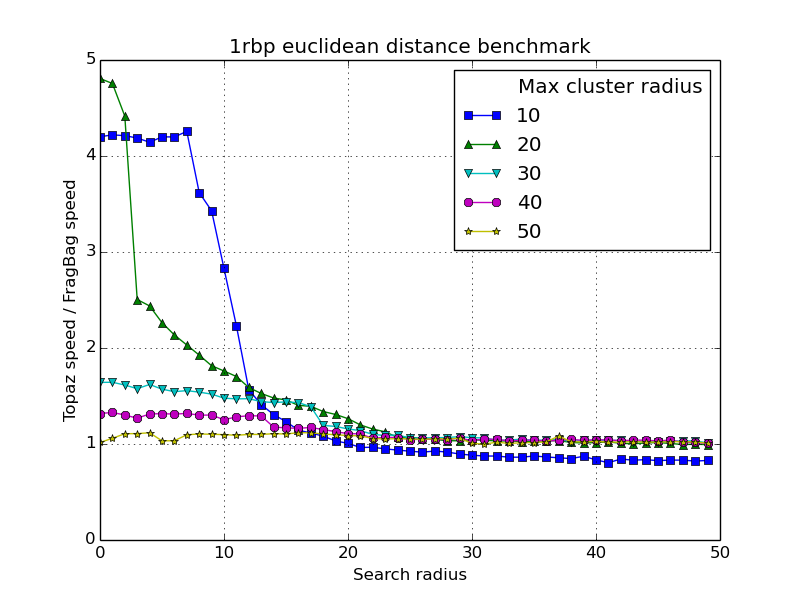
\includegraphics[width=1\textwidth]{assets/1rbp_euclid.png}
        %\caption{}
    \end{subfigure}
    \caption{FragBag benchmarking data. (a) Cosine distance gives on the whole better acceleration, but results in only $>99.8\%$ sensitivity, whereas (b) Euclidean distance as a metric is guaranteed by the Triangle Inequality to get $100\%$ sensitivity.}
    \label{fig:fragbag}
\end{figure}


\subsubsection{Validation}
Note that while Euclidean distance is a metric, and thus the triangle inequality guarantees 100\% sensitivity, cosine distance is not.
Empirically, however, for all of the queries we performed, we achieve $> 99.8\%$ sensitivity (Table \ref{tab:fragbag_cosine_sensitivity}).
Full results for each data point can be found in supplementary data files.

\begin{table}
    \centering
    \caption{Average sensitivity of Topaz compared to FragBag when using cosine distance for the trials described in Figure \ref{fig:fragbag_cosine}. This table averages the sensitivities for each choice of search radii $\{0, 0.01, \ldots, 0.49\}$. (NB: no analogous table is given for euclidean distance as the Triangle Inequality ensures perfect recall).}
    \label{tab:fragbag_cosine_sensitivity}
    \begin{tabular}{|c|cccc|}
        \hline
        \backslashbox{Cluster radii}{Query protein}  & 4rhv & 1ake & 1bmf & 1rbp \\
        \hline
        0.10  & 1  & 0.999840     & 0.998490 & 0.999950  \\
        0.20  & 1  & 0.999918     & 0.999001 & 0.999978  \\
        0.30  & 1  & 0.999926     & 0.999649 & 1  \\
        0.40  & 1  & 0.999974     & 0.999796 & 1  \\
        0.50  & 1  & 0.999984     & 0.999934 & 1  \\
        \hline
    \end{tabular}
\end{table}

\section{Discussion}

We have introduced a data structure for accelerating approximate search, and
demonstrated its effectiveness in three distinct areas of computational
molecular biology.
This data structure provably scales almost linearly with entropy of the 
database, allowing search on large data sets to scale even as these data sets
grow exponentially.
We provide open-source software for all three areas: caBlastX for metagenomic analysis,
Ammolite for small-molecule structure search, and Topaz for protein structure search.
In the case of metagenomic analysis, caBLASTX also compares favorably to recent 
search tools that outperform BLASTX.

In this work, we have not focused on the space-saving compression that is
possible with entropy-scaling data structures, but rather on the run-time
acceleration of approximate search.
However, particularly in the case of metagenomic analysis, the collection of 
read data presents a problem for storage and transfer, as well as analysis.

\section{Online Methods}

\subsection{Theory}
\subsubsection{Time-complexity}
Recall our definition of the entropy-scaling similarity search data structure (Figure \ref{fig:dataStructure}).
For ease of analysis, we will work in a high-dimensional metric space and consider the database as a set $D$ of $n$ unique points in that metric space.
Note however that the metricity requirement is needed only for a 100\% sensitivity guarantee; other distance functions can be used, but result in some loss in sensitivity.
However, regardless of the distance function chosen, there cannot be a loss of
specificity; false positives will never be introduced.
\hl{NMD: should we bother to prove this?}
Define $B_S(q,r) = \{ p \in S | ||q-p||<r \}$. The similarity search problem is thus to compute $B_D(q,r)$ for a query $q$ and radius $r$.

The data structure first clusters the points in the set by assigning them to their nearest `cluster center'.
A set $C$ of $k$ cluster centers are chosen such that no cluster has radius greater than a user-specified parameter $r_c$ and no two cluster centers are within distance $r_c$ of one another.
Overloading notation a bit, we will identify each cluster with its center, so $C$ is also the set of clusters.
%We will additionally require that each cluster contain at least $\frac{n}{k \alpha}$ items, for some constant $\alpha \ge 1$ (i.e. that the clusters are balanced).
For a given similarity search query of all items within distance $r$ of a query $q$, this data structure breaks the query into coarse and fine search stages.
The coarse search is over the list of cluster centers, returning $B_C(q,r + r_c)$.
Let \[\displaystyle F = \bigcup_{c \in B_C(q,r+r_c)} c , \] the union of all the returned clusters.
Then by the triangle inequality, $B_F(q,r) = B_D(q,r)$.
Thus, a fine search over the set $F$ can return all items within radius $r$ of $q$.

Note that we require the metricity requirement only for the Triangle Inequality.
It turns out that many interesting distance functions are not metrics, but still almost satisfy the Triangle Inequality, which is nearly sufficient.
More precisely, if an $\alpha$ fraction of the triples in $S$ do not satisfy the Triangle Inequality, then in expectation, we will have sensitivity $1 - \alpha$.
As we will see later, empirically, this loss in sensitivity appears to be low, and can likely be ameliorated by increasing the coarse search radius.

%We will prove in this section that 
This data structure allows for similarity search queries in time roughly linear (provided the fractal dimension of the database is low) to the metric entropy of the database.
Additionally, under some uniformity assumptions, the data structure can be stored in a compressed form that uses space also linear in the metric entropy of the database.
Further, as suggested by the last sentence, the metric entropy of the database can be related to the more typical information theoretic notion of entropy (see Online Methods).
%However, to do this, we will first need to build additional mathematical machinery and make precise our notions of `entropy' and `fractal dimension'.

Note that entropy-scaling data structures are distinct from both succinct data structures and compressed data structures.
Succinct data structures are ones that use space close to the information-theoretic limit in the worst case while permitting efficient queries; i.e.
succinct data structures do not depend on the actual entropy of the underlying data set, but have size-dependence on the potential worst-case entropy of the data set \cite{jacobson1988succinct}.
Compressed (and opportunistic) data structures, on the other hand, bound the amount of the space used by the entropy of the data set while permitting efficient queries \cite{grossi2005compressed, ferragina2000opportunistic}.
Entropy-scaling data structures are compressed data structures, but can do even more, as
unlike entropy-scaling data structures though, compressed data structures do not measure time-complexity in terms of the entropy.
\textbf{The primary theoretical advance of entropy-scaling data structures is that they bound both space and time as functions of the data set entropy.}

\subsubsection{Complexity bounds}
We first define the concept of metric entropy and entropy dimension as is usual in fractal geometry:
\begin{definition}[\cite{tao2014metric} Definition 3] 
    Let $X$ be a metric space, let $D$ be a subset of $X$, and let $\rho>0$ be a radius.
    \begin{itemize}
        \item The \textit{internal covering number} $N_\rho^{int}(D)$ is the fewest number of points $x_1, \ldots, x_n \in D$ such that the balls $B(x_1,\rho), \ldots B(x_n,\rho)$ cover $D$.
        \item The \textit{metric entopy} $N_\rho^{ent}(D)$ is the largest number of points $x_1, \ldots, x_n$ one can find in $D$ that are $\rho$-separated, thus $||x_i - x_j|| \ge \rho$ for all $i \ne j$.
    \end{itemize}
\end{definition}
\begin{definition}[\cite{falconer2013fractal}]
    The upper Minkowski dimension (also known as the entropy dimension) of a set $D$ is given by 
\[
    \dim_{Minkowski}(D) := \limsup_{\rho \to 0} \frac{\log N_\rho(D)}{\log 1/\rho}
\]
\end{definition}
Unfortunately, as $D$ is a finite, discrete, set, the given definision always gives $\dim_{Minkowski}(D) = 0$.
However, we are only interested in scaling behaviors around large radii, so instead we use:
\begin{definition}
    The fractal dimension $d$ of a set $D$ at a scale $[\rho_1,\rho_2]$ is given by
    \[
        d = \operatorname*{arg\,max}_{d^*} \{ N_\rho(D) \propto \rho^{-d^*} | \rho \in [\rho_1,\rho_2] \}.
    \]
\end{definition}

Recall that $k$ entries are selected as cluster centers for partitioning the database to result in clusters with maximum radius $r_c$.
From the definition above, it is trivial to verify $ N_{r_c}^{int}(D) \le k \le N_{r_c}^{ent} (D)$.
The upper bound is guaranteed by our requirement that the cluster centers not be within distance $r_c$ and the lower bound follows from the fact that our clustering is designed to cover the database.

%We will set $r_c = \theta(\frac{1}{k})$.
Given any query $q$, the coarse search over the cluster centers always requires $k$ comparisons.
Additionally, the fine search is over the set $F$, the union of clusters with centers within distance $r+r_c$ from $q$.
As the time-complexity of similarity search is just the total of the coarse and fine searches, this implies that the total search time is $O(k + |F|)$.

By the triangle inequality, $F \subset B_D(q,r+r_c)$,
so we can bound $|F| \le |B_D(q,r+r_c)|$.
Let the fractal dimension $D$ at the scale between $r_c$ and $r_c + r$ be $d$.
Then in expectation over possible queries $q$,
\[
    \left|B_D(q, r+r_c)\right| \sim \left|B_D(q,r)\right|\left(\frac{r+r_c}{r}\right)^d .
\]
Roughly speaking, this scaling argument just says that doubling a search radius only increases the number of hits by a factor of at most $2^d$.
Thus, total search time is 
\[
    O\left(k + \left|B_D(q,r)\right|\left(\frac{r+r_c}{r}\right)^d \right).
\]
However, note that $k$ is linear in metric entropy and $|B_D(q,r)|$ is the output size, so similarity search can be performed in time linear to metric entropy and a polynomial blow-up of output size.
Provided that the fractal dimension $d$ is small and $k$ is large, the search time will be dominated by the metric entropy component, which turns out to be the regime of greatest interest for us.

We have thus proven bounds for the time-complexity of similarity search.
Next, we also prove space-complexity bounds for the data structure and connect metric entropy with information-theoretic entropy under some additional uniformity assumptions.

\subsubsection{Space-complexity}
Here we bound the space-complexity of our entropy-scaling data structure and show that metric entropy bounds can give information-theoretic Shannon entropy bounds.
To do this, we will need two conditions: (1) that our distance function measures marginal entropies and (2) that all clusters are smaller than some constant $S_c$.

Information-theoretic ``entropy'' is of course a measure of the uncertainty of a distribution or random variable, and is not well-defined for a database.
However, the term is often used in data compression as a shorthand for the number of bits needed to encode the database, a measure of the randomness of that database.
We use entropy in the latter sense; precisely, we define the entropy of a database as the number of bits needed to encode the database under some encoding scheme.
Equivalently, the entropy of a database is the entropy measured in bits of a random variable whose instances are databases that match our database on some structural condition, which we will define later.
Of course, each encoding scheme thus results in a different definition of entropy, but this simply corresponds to the compressed size of the database under different compression methods.
We now estimate the entropy of the database by attempting to compress it.

Let $l$ be the number of bits necessary to encode a point $p$ in the space \textit{de novo} without any other information.
Without any compression, a set of size $n$ then requires $nl$ bits to store.
Assume that the number of bits necessary to encode a point $p$ as a function of $q$ (and vice versa) is $\theta(||p-q||) \le l$.
Effectively, we are imposing the condition that the distance is a measure of entropy added by a new point (`pairwise marginal entropy').
That distance bounds pairwise marginal entropy is clearly true for Hamming distance, and can also be shown for edit distances and more general similarity measures.

Let us consider the spanning trees of the complete distance graph between points in the set.
The number of bits needed to encode the entire set according to the relationships specified in the spanning tree is then linear in the weight of that tree.
Thus, the weight of a spanning tree effectively corresponds to the entropy of the distribution over all data sets that are in accordance with the pairwise distances specified in that tree.
One measure of the entropy of a data set would be the entropy of this distribution over a minimum weight spanning tree of the complete distance graph, and let us call that weight $W_1$.
However, we have neglected the number of bits needed to encode the tree itself; as this is an arbitrary tree, every node must encode its parent, so the entropy of the tree itself is $ (n-1) \log n$ bits.
Thus, this encoding is not practical as encoding the tree is already super-linear in data set size.
In total, including encoding the root node, the database will require $O(l + W + (n-1)\log n$ bits to store.

Alternately, we can also specify a set of $k$ privileged points using which we encode all other points, corresponding to our cluster centers.
With the additional selection of an arbitrary (or zero) root node, this encoding corresponds to a 2-level spanning tree of the complete distance graph, with pre-selected branches, but leaves selected to minimize total weight.
Obviously, the weight of this 2-level spanning tree $W_2 \ge W_1$, but
encoding the tree itself uses only $kl$ bits to specify each of the privileged points and $n \log k$ to encode the tree the cluster identifications.
Thus, the database will require $O(kl + W_2 + n \log k)$ bits to store.
%This model of entropy also has the advantage of being much more amenable for proving bounds about the time- and space-complexity of the similarity search data structure we introduce below.
However, the cluster identifications can be encoded positionally on disk, so we can actually store it in just $O(kl + W_2)$ bits, so the data structure is basically linear in the entropy of a distribution corresponding to a 2-level cluster.

It turns out though, that we can often do even better than that given a metric entropy $N_{r_c}^{ent} = k$, and actually bound the tree weight $W_3$ with a slightly different tree structure.
Recall that we assumed the maximum cluster size $S_c$, and the maximum cluster radius is $r_c$ if $k$ points chosen to be at least distance $r_c$ from each other are used as the cluster centers.
We now consider encoding each item by its nearest neighbor within a cluster, which corresponds to a tree made by joining together a forest of minimum spanning trees corresponding to each individual cluster by the roots (i.e. cluster centers).
Clearly, this decreases the weight of the tree from the previous 2-level spanning tree, so $W_1 \le W_3 \le W_2$.
As each cluster has at most $S_c$ elements, encoding the tree itself uses $(n-k)\log S_c$, but specifying the privileged points again requires $kl$ bits.
Thus, total number of bits needed is $O(kl + W_3 + (n-k)\log S_c )$

But because the cluster sizes are bounded by $S_c$, we can effectively still encode positionally by using a large window and a standard text compressor like Gzip or Bzip2 and setting the compression window to be larger than $S_c l$.
Instead of directly encoding differences, this scheme instead lists all cluster members together and uses a standard text compressor to use the redundancy throughout the cluster, which allows us to not store the forest explicitly and still get compression.
Thus, the total number of bits needed is roughly $O(kl + W_3)$. Again, we can get a data structure basically linear in the entropy, but here linear in the entropy of a distribution closer to that of the optimal minimum spanning tree.

Furthermore, we can additionally bound the entropy $W_3$ using the metric entropy $k$.
Because maximum cluster radius is $r_c$, the entropy added to the cluster from any individual item is $O(r_c)$.
Additionally, each cluster is of size at most $S_c$, so each cluster has $O(r_c \cdot S_c)$ bits of entropy.
Thus, $W_3 = O(k r_c S_c)$.
Or, alternately, each individual item must fall in a cluster, so we can also bound $W_3 = O(n r_c)$.
In this manner, we can relate the Shannon entropy of the database to the metric entropy that we used in the time-complexity bounds.

\subsection{Cablastx}

\subsubsection{Alphabet Reduction}

Alphabet reduction--reducing the 20-letter standard amino acid alphabet to a
smaller set, in order to accelerate search or improve homology detection--has
been proposed and implemented several times~\cite{bacardit2007automated, peterson2009reduced}.
In particular, \citet{murphy2000simplified} considered reducing the
amino-acid alphabet to 17, 10, or even 4 letters.
More recently, \citet{zhao2012rapsearch2} and \citet{huson2013poor} applied a reduction to
a 4-letter alphabet, termed a ``pseudoDNA'' alphabet, in sequence alignment.

In this work, we extend the compression approach of 
\citet{daniels2013compressive} using a reversible alphabet reduction.
We use the alphabet reduction of \citet{murphy2000simplified} to map the 
standard amino
acid alphabet (along with the four common ambiguous letters ) onto a 4-letter 
alphabet.
Specifically, we map F, W, and Y into one cluster; C, I, L, M, V, and J into
a second cluster, A, G, P, S, and T into a third cluster, and
D, E, N, Q, K, R, H, B, and Z into a fourth cluster.
By storing the offset within each cluster of the original letter, the original
sequence can be reconstructed, making this a reversible reduction.

\subsubsection{Database Compression}

Given a protein sequence database to be compressed, we proceed as follows:
\begin{enumerate}
        \item First, initialize a table of all possible $k$-mer ``seeds'' of
        our 4-letter reduced alphabet, as well as a ``coarse'' database of
        reduced-alphabet sequences, initially containing the alphabet-reduced
        version of the first sequence in the input database.
        %
        \item For each $k$-mer of the first sequence, store its position in the
        corresponding entry in the seed table.
        %
        \item For each subsequent sequence $s$ in the input, slide a window of 
        size $k$ along the sequence, skipping single-residue repeats of length
        greater than 10.
        %
        \item Look up these $k$ residues in the seed table.
        For every entry matching to that $k$-mer in the seed table, follow
        it to a corresponding subsequence in the coarse database and attempt
        \textit{extension}.
        If no subsequences from this window can be extended, move the window
        by $m$ residues, where $m$ defaults to 10.
        \item If a match was found via extension, move the $k$-mer window to
        the first $k$-mer in $s$ after the match, and repeat the extension
        process.
\end{enumerate}
        
Given a $k$ match between sequence $s$ and a subsequence $s'$ pointed to by the
seed table, first attempt \textit{ungapped} extension:
\begin{enumerate}
        \item Within each window of 10 alphabet-reduced residues, if identical 
        4-mers in $s$ and $s'$ can be found, and at least 2 additional matching 
        residues can be found, then there is an ungapped match within that
        10-mer window between $s$ and $s'$ that exhibits at least 60\% sequence
        identity.
        \item Continue ungapped matching using 10-mer windows until no more
        10-mers of at least 60\% sequence identity are found.
        \item The result of ungapped extension is that there is an alignment 
        between $s$ and $s'$ where the only differences are substitutions,
        at least 60\% of the positions contain exact matches.
\end{enumerate}
        
When ungapped extension terminates, attempt \textit{gapped} extension.
From the end of the aligned regions thus far, align 25-mer windows of both
$s$ and $s'$ using the Needleman-Wunsch~\cite{needleman1970general} algorithm 
using an identity matrix.
Note that the original caBLASTP~\cite{daniels2013compressive} used BLOSUM62 as 
it was
operating in amino acid space; as we are now operating in a reduced-alphabet
space, an identity matrix is appropriate, just as it is for nucleotide space.
After gapped extension on a window length of 25, attempt ungapped extension
again.

If neither gapped nor ungapped extension can continue, end the extension phase.
If the resulting alignment has less than 70\% sequence identity (in the 
reduced-alphabet space), or is shorter than 40 residues, discard it, and 
attempt extension on the next entry in the seed table for the original $k$-mer,
continuing on to the next $k$-mer if there are no more entries.

If the resulting alignment does have at least 70\% sequence identity in the
reduced-alphabet space, and is at least 40 residues long, then create a link
from the entry for $s'$ in the coarse database to the subsequence of $s$
corresponding to the alignment.
If there are unaligned ends of $s$ shorter than 30 residues, append them to the
match.
Longer unaligned ends that did not match any subsequences reachable from the
seed table are added into the coarse database themselves, following the same
$k$-mer indexing procedure as the first sequence.

Finally, in order to be able to recover the original sequence with its original
amino acid identities, a \textit{difference script} is associated with each
link.
This difference script is a representation of the insertions, deletions, and
substitutions resulting from the Needleman-Wunsch alignment, along with the
offset in each reduced-alphabet cluster needed to recover the original alphabet.
Thus, for example, a valine (V) is in the cluster containing C, I, L, M, V, and 
J.
Since it is the 4th entry in that 5-entry cluster, we can represent it with
the offset 4.
Since the largest cluster contains 9 elements, only four bits are needed to
store one entry in the difference script.
More balanced clusters would have allowed 3-bit storage, but at the expense of
clusters that less faithfully represented the BLOSUM62 matrix and the
physicochemical properties of the constituent amino acids.

\subsubsection{Further benchmarking and validation}

Although our primary result is the direct acceleration of BLASTX using our
entropy-scaling data structures, we also compared caBLASTX to 
RapSearch2~\cite{zhao2012rapsearch2} version 2.22 and the November 29, 2014 
version of Diamond~\cite{buchfink2014fast}.
All tests were performed on a 12-core Intel Xeon X5690 running at 3.47GHz with
88GB RAM and hyperthreading; 24 threads were allowed for all programs.
Both Diamond was run with the \texttt{--sensitive} option.
In all cases, an E-value threshold of \texttt{1e-7} was used.

\begin{table}
\caption{Running time of BLASTX, caBLASTX, RapSearch2, and Diamond. All units in seconds.\label{mgspeed}}
\begin{tabular}{ccccc}
\hline
dataset & BLASTX & caBLASTX & RapSearch2 & Diamond \\
\hline
assemblies & 3235 & 123 & 194 & 50 \\
\hline
NGS reads & 14423 & 21 & 51 & 13 \\
\hline
\end{tabular}
\end{table}

\begin{table}
\caption{Accuracy of caBLASTX, RapSearch2, and Diamond.\label{mgacc}}
\begin{tabular}{cccc}
\hline
dataset & caBLASTX & RapSearch2 & Diamond \\
\hline
assemblies & 99.2\% & 87.7\% & 91.0\% \\
\hline
NGS reads & 95.7\% & 79.5\% & 76.9\% \\
\hline
\end{tabular}
\end{table}

While Diamond is notably faster than caBLASTX, it achieves this speed at the
expense of some accuracy, particularly on raw reads.
Moreover, caBLASTX actually accelerates standard BLASTX itself, and allows the
user to pass arbitrary parameters to the underlying BLASTX during fine search.
Thus, caBLASTX may be suitable to a wider variety of existing analysis 
pipelines.
With respect for future work, it may be possible to apply entropy-scaling data
structures to Diamond itself, achieving even greater speed gains.
Of course, the accuracy of such an approach would still be limited by Diamond; 
entropy-scaling data structures cannot themselves improve accuracy,
except by virtue of making computationally expensive analyses more tractable.

CaBlastx is implemented in Go, and its source code is available on Github.

\subsection{Ammolite}

\subsubsection{Simplification and compression}

First, we remove hydrogen atoms from the molecules; hydrogens can be easily recovered by inferring their 
presence.
Next, each molecule's graph structure is converted to an unlabeled one; each atom label is removed, and each
bond type is represented as just a single bond.
The removed information--atom and bond type--is stored in an auxiliary data structure, indexed by the molecule's
PubChem ID and the atom or bond number.
Next, any vertex or edge that is not part of a simple cycle or a tree is removed, and any edge that is part
of a tree is removed.
This preserves the node count, but not the topology, of tree-like structures, and preserves simple cycles,
which represent rings in chemical compounds.
For example, as shown in Figure~\ref{}, bicyclohexyl and dicyclohexylamine would appear identical.

After this transformation is applied to each molecule in a database to be compressed, we identify all clusters
of fully-isomorphic transformed molecular graphs.
Isomorphism detection is performed using the VF2~\cite{cordella2001improved} 
algorithm; a simple hash computed from the
number of vertices and edges in each transformed molecular graph is first used 
to filter molecular graphs that cannot possibly be isomorphic.
A representative from each such cluster is stored in SDF format; collectively, these representatives form a 
``coarse'' database.
Along with each representative, we preserve the information necessary to reconstruct each original molecule,
as a pointer to a set of vertices and edges that have been removed or unlabeled.

Ammolite is implemented in Java, and its source code is available on Github.

\subsection{Topaz}
We took the existing FragBag method as a black box and by design did not do anything clever in Topaz except apply our entropy-scaling similarity search data structure.
Additionally, we removed the sorting-by-distance feature of Andrew Gallant's 
FragBag search function, which does not improve the all-matching results we 
were interested in here---it lowers $k$-nearest neighbor search memory 
requirements while dominating the running time of $\rho$-nearest neighbor, the 
problem at hand.
This was done for both the FragBag and the Topaz benchmarks, to ensure comparability.
All code was written in Go, and is available on Github.

The entire 2014 Oct 31 version of the Protein Data Bank was downloaded and the 
database was composed of fragment frequency vectors generated from all of the 
relevant PDB files using the 400-11.json fragment list, as described in \citep{budowski2010fragbag}.
For this paper, we implemented the benchmarking in Go, and have provided the 
source code for the benchmarking routine.
This allowed us to benchmark just the search time, excluding the time to load the database from disk.
The prototype implementation of Topaz is also available, but only supports the 
all $\rho$-nearest neighbor search query found in FragBag.

\section{Author Contributions}
Y.W.Y., N.M.D. and B.B. conceived the project.
Y.W.Y. developed the theoretical analyses, with help from N.M.D.
N.M.D. implemented and benchmarked Cablastx.
D.C.D. implemented and benchmarked Ammolite, with help from N.M.D.
Y.W.Y. applied the entropy-scaling data structure to accelerate FragBag, with help from N.M.D.
B.B. supervised research and provided critical advice on the study.
Y.W.Y., N.M.D. and B.B. wrote the manuscript.

\section{Acknowledgments}
Y.W.Y. is supported by a Hertz Foundation fellowship.
N.M.D. is supported by \hl{(big data grant)}.
We thank Andrew Gallant for his implementation of Fragbag.

\bibliographystyle{model2-names}
%\bibliographystyle{plain}
\bibliography{main}

\newpage

\appendix
\section{Extraneous}
\subsection{Random text}

Faster approximate string matching over compressed text \cite{navarro2001faster}.
Approximate Searching on Compressed Text \cite{perez2005approximate}.
A Text Compression Scheme That Allows Fast Searching Directly In The Compressed File \cite{manber93atext}.
\begin{itemize}
\item Approximate search on compressed data is designed for a linear text, and is specific to edit distances.
\end{itemize}

Adaptive Cluster Distance Bounding for High-Dimensional Indexing \cite{ramaswamy2011adaptive}
\begin{itemize}
\item I don't think their method works well for Hamming-like distances, as
   their hyperplane separation method seems like it ought to work best
   in Euclidean-like spaces? They certainly only use very continuous
   spaces in their examples.
\item Their "compressed feature vectors" don't actually have anything to do
   with entropy, as it looks like a constant binning.
\item Because their distances are Euclidean, they didn't (and most likely
   couldn't) make a connection we're making between clustering and
   entropy/compression. Thus, their data structure still uses $O(n)$
   space, while ours can use $O(H(n))$ space, where $H(n)$ is the "entropy"
   of the dataset.
\item They didn't do a full analysis of how much clustering helps them,
   though they mention that it does and have empirical experiments.
\item They are working on the k-nearest neighbor problem, not the
   $\epsilon$-nearest neighbors problem that we are. However, their method
   certainly can be adapted to $\epsilon$-nearest neighbor, nearly
   trivially.
\end{itemize}

\subsection{Technical details and motivation for the similarity search data structure}
Let us provide a bit more motivation and rigorous analysis for the general entropy-scaling similarity search data structure.
Consider the cost of querying a database of size $n$ for all entries within some distance $r$ of some query item $q$.
All database entries and the query are drawn from a universe $U$ of possible elements, and we impose on the database both a sparsity assumption and a strong structural assumption (described below).
%For ease of analysis, we will also assume here that the distance function is a metric, but this metricity assumption can be relaxed.

%The quantitative form of knowledge we are most interested in encoding is pairwise distance from the query.
%Of course, that knowledge is already implicitly available in the database through computing pairwise distance from the query as needed.
%Indeed, this is the most commonly used naive method, but it turns out to be an expensive endeavor, scaling linearly with the size of the database.
The most commonly used na\"ive method is to simply compute pairwise distance from the query as needed.
This is easy, but requires a linear scan through the entire database, which itself uses also linear space.
Unfortunately, this can often be prohibitively slow.

One other naive approach is to pre-compute and sort all pairwise distances between database entries and potential queries into a rainbow table.
If we are given the guarantee that the space of potential queries is small, this approach might be feasible, as then a query requires only a single lookup and effectively constant time to traverse the list of sorted distances until all database entries within $r$ of the query are recovered.
However, in practice, we do not know in advance the queries expected, and thus constructing such a table requires memory $O(n|U|)$ and time $O(n \log n |U|)$, which is undesirable as the database in sparse in $U$, so $|U| >>n$.

Unlike cryptographic hash functions (for which rainbow tables are actually used \cite{oechslin2003making}, the outputs for similar queries in similarity search are strongly correlated.
We can easily take advantage of these correlations by instead storing the pairwise distances among just the database entries in a self-similarity table.
Then, if we are really lucky and the query is a database entry, we only have to do the same constant-time lookup as in the rainbow table.
Most of the time, however, we will not be so lucky, and the query will not be a database entry.

For the general case when the query is not a database entry, let us label the database entries $d_1, \ldots, d_n$.
WLOG, all of these are \textit{a priori} equivalent; say we first compare $q$ to $d_1$ by looking at the first row of the table.
Then by the triangle inequality, all database entries within radius $r$ of $q$ must be within distance $||q-d_1|| +r$ of $d_1$.
Thus, if $q$ is close to $d_1$, we need only check some small fraction of the database.
If $d_1$ is far from $q$, we can instead progressively try other rows, starting with $d_2, d_3$, etc.
(note that we will call $d_i$ the central element of row $i$).
Without going into detail, it is intuitively obvious that the closer together (more redundant) database entries are, the better the performance of similarity search on this data structure, and thus we begin to scale with entropy.
However, constructing this data structure still requires memory-complexity of $O(n^2)$ and time-complexity $O(n^2 \log n)$, which is still not ideal.

Note that there are still three major sources of extraneous information in the pairwise distances table:

\begin{enumerate}
    \item We have $n$ copies of the database, one copy for each database entry.
However, the algorithm will almost never get to the end of the table, because it will likely contain a sufficiently close starting database entry before then, so the last rows are probably unnecessary.
    \item Similarly, the last columns of each row are also probably unnecessary, as the algorithm only cares about entries that are close to the central entry of the row.
    \item The sorting information within each row is used to check only if entries fall within a particular radius and not used beyond that.
\end{enumerate}

It is by eliminating this extraneous information that we constructed a generalized data structure we introduced in the paper.
More precisely, we reduce the table to $k$ rows.
Then, we remove all the ``distant'' entries from every row, so that every database entry appears in only one row, the one to whose central element it is closest.
Additionally, we do not need the full sorting information, since each entry only appears with its closest row center.
Note that the data structure is no longer a table, but rather instead a partition of the original database, thus instead of rows, we refer to clusters and cluster centers.
Say that the maximum cluster radius is $r_c$.
Then the similarity search algorithm is to do a `coarse search' on the cluster centers for all centers within distance $r+r_c$ of $q$, expand those clusters, and do a ‘fine search’ on all entries in those clusters for those entries within distance $r$ of $q$, as stated earlier.

\end{document}

